\vspace*{40mm}
\begin{center}
\Large\bfseries DREIECKSKRANZ UM OLDENBURG.
\end{center}
\vfill
\noindent IX.\hfill42
\clearpage\null\clearpage
\begin{landscape}
\begin{center}
\Large\bfseries NACHLASS.
\end{center}
\begin{center}
\bfseries Zur Ausgleichung des Dreieckskranzes, der das Oldenburger Gebiet umgibt.
\end{center}
\par\noindent\hspace*{\parindent}Die ursprüngliche Tabelle ist an die Seite Zeven-Steinberg angeschlossen,
[deren] vorausgesetzter Azimut in der Ebene \(1^{0}\,17'\,40''{,}568\) und deren logDist \(4{,}523\,5878\) betragen.
In der folgenden Tabelle sind alle Azimute auf die Ebene reduziert.
\par\medskip
\begingroup
\small
\setlength{\tabcolsep}{3pt}
\renewcommand{\arraystretch}{1.05}
\noindent
\begin{minipage}[t]{.32\linewidth}\centering
\begin{tabular}{r|rrr|r||}
&\multicolumn{3}{c|}{\shortstack{[Ebener\\Beobachtungsw.]}}&[1. Ausgl.]\\[4pt]
&\multicolumn{3}{c|}{\textbf{1. Zeven}}&\\[3pt]
2&\(1^{0}\)&\(17'\)&\(39''{,}871\)&\(40''{,}568\)\\
21&53&26&5,943&5,235.5\\
20&124&13&47,140&47,150.5\\[6pt]
&\multicolumn{3}{c|}{\textbf{2. Steinberg}}&\\[3pt]
3&36&16&55,159&57,067\\
21&106&46&4,198&2,987\\
1&181&17&41,266&40,569\\[6pt]
&\multicolumn{3}{c|}{\textbf{3. Asendorf}}&\\[3pt]
5&25&49&22,245&24,092\\
4&98&13&54,829&55,023\\
21&159&2&46,795&46,682\\
2&216&16&58,976&57,068\\[6pt]
&\multicolumn{3}{c|}{\textbf{4. Twistringen}}&\\[3pt]
6&47&24&55,642&56,367.5\\
21&200&32&28,288&27,951\\
3&278&13&55,217&55,023\\
5&330&2&34,130&33,935.5\\[6pt]
&\multicolumn{3}{c|}{\textbf{5. Knickberg}}&\\[3pt]
7&37&16&32,547&33,219.5\\
6&87&27&23,007&23,987\\
4&150&2&33,742&33,936.5\\
3&205&49&25,941&24,094
\end{tabular}
\end{minipage}\hfill
\begin{minipage}[t]{.32\linewidth}\centering
\begin{tabular}{r|rrr|r||}
&\multicolumn{3}{c|}{\shortstack{[Ebener\\Beobachtungsw.]}}&[1. Ausgl.]\\[4pt]
&\multicolumn{3}{c|}{\textbf{\shortstack{6. Mordkuhlen-\\berg}}}&\\[3pt]
8&\(16^{0}\)&\(10'\)&\(32''{,}113\)&\(32''{,}784\)\\
9&88&47&59,913&61,059.5\\
10&160&48&58,348&59,114.5\\
4&227&24&57,094&56,368.5\\
5&267&27&24,968&23,988\\
7&332&14&35,728&34,849.5\\[6pt]
&\multicolumn{3}{c|}{\textbf{7. Nonnenstein}}&\\[3pt]
8&73&3&40,746&40,540\\
6&152&14&33,970&34,848.5\\
5&217&16&33,892&33,219.5\\[6pt]
&\multicolumn{3}{c|}{\textbf{8. Dörenberg}}&\\[3pt]
9&155&5&19,362&19,827\\
6&196&10&33,455&32,784\\
7&253&3&40,334&40,540\\[6pt]
&\multicolumn{3}{c|}{\textbf{9. Quekenberg}}&\\[3pt]
11&159&44&54,268&55,012.5\\
10&210&48&6,055&6,922\\
6&268&48&2,206&1,059.5\\
8&335&5&20,293&19,828
\end{tabular}
\end{minipage}\hfill
\begin{minipage}[t]{.32\linewidth}\centering
\begin{tabular}{r|rrr|r}
&\multicolumn{3}{c|}{\shortstack{[Ebener\\Beobachtungsw.]}}&[1. Ausgl.]\\[4pt]
&\multicolumn{3}{c|}{\textbf{10. Krapendorf}}&\\[3pt]
9&\(30^{0}\)&\(48'\)&\(7''{,}788\)&\(6''{,}921\)\\
11&98&33&4,402&4,679\\
12&172&39&16,470&17,826.5\\
6&340&48&59,881&59,114.5\\[6pt]
&\multicolumn{3}{c|}{\textbf{11. Windberg}}&\\[3pt]
13&174&6&1,682&2,017.5\\
12&214&9&23,903&24,589\\
10&278&33&4,956&4,679\\
9&339&44&55,757&55,012.5\\[6pt]
&\multicolumn{3}{c|}{\textbf{12. Westerstede}}&\\[3pt]
11&34&9&25,276&24,590\\
13&86&4&31,500&31,113\\
14&130&8&55,475&55,597.5\\
15&178&53&40,498&41,124\\
16&223&18&2,675&4,356\\
10&352&39&19,183&17,826.5\\[6pt]
&\multicolumn{3}{c|}{\textbf{13. Leer}}&\\[3pt]
14&186&16&22,030&21,978.5\\
12&266&4&30,726&31,113\\
11&354&6&2,354&2,018.5
\end{tabular}
\end{minipage}
\par\endgroup
\vfill\hfill\(42^{*}\)
\clearpage
\noindent332\hfill\textbf{NACHLASS.}
\par\bigskip
\begingroup
\small
\setlength{\tabcolsep}{3pt}
\renewcommand{\arraystretch}{1.1}
\noindent
\begin{minipage}[t]{.32\linewidth}\centering
\begin{tabular}{r|rrr|r||}
&\multicolumn{3}{c|}{\shortstack{[Ebener\\Beobachtungsw.]}}&[1. Ausgl.]\\[4pt]
&\multicolumn{3}{c|}{\textbf{14. Aurich}}&\\[3pt]
13&\(6^{0}\)&\(16'\)&\(21''{,}927\)&\(21''{,}978.5\)\\
15&249&39&8,645&8,716\\
12&310&8&55,720&55,597.5\\[6pt]
&\multicolumn{3}{c|}{\textbf{15. Jever}}&\\[3pt]
14&69&39&8,787&8,716\\
17&263&59&50,022&50,186.5\\
16&322&58&6,388&6,920.5\\
12&358&53&41,751&41,125\\[6pt]
&\multicolumn{3}{c|}{\textbf{16. Varel}}&\\[3pt]
12&43&18&6,038&4,357\\
15&142&58&7,453&6,920.5\\
17&207&44&1,620&1,240\\
18&239&21&2,220&2,335.5\\
19&292&10&0,264&2,742
\end{tabular}
\end{minipage}\hfill
\begin{minipage}[t]{.32\linewidth}\centering
\begin{tabular}{r|rrr|r||}
&\multicolumn{3}{c|}{\shortstack{[Ebener\\Beobachtungsw.]}}&[1. Ausgl.]\\[4pt]
&\multicolumn{3}{c|}{\textbf{17. Langwarden}}&\\[3pt]
16&\(27^{0}\)&\(44'\)&\(0''{,}860\)&\(1''{,}240\)\\
15&83&59&50,352&50,187.5\\
18&283&31&20,848&20,632.5\\[6pt]
&\multicolumn{3}{c|}{\textbf{18. Bremerlehe}}&\\[3pt]
16&59&21&2,451&2,335.5\\
17&103&31&20,418&20,633.5\\
20&304&0&38,544&38,541.5\\
19&347&18&42,192&42,094.5\\[6pt]
&\multicolumn{3}{c|}{\textbf{19. Garlste}}&\\[3pt]
16&112&10&5,220&2,742\\
18&167&18&41,997&42,094.5\\
20&229&19&45,572&46,317\\
21&345&11&48,789&50,424.5
\end{tabular}
\end{minipage}\hfill
\begin{minipage}[t]{.32\linewidth}\centering
\begin{tabular}{r|rrr|r}
&\multicolumn{3}{c|}{\shortstack{[Ebener\\Beobachtungsw.]}}&[1. Ausgl.]\\[4pt]
&\multicolumn{3}{c|}{\textbf{20. Brillit}}&\\[3pt]
21&\(19^{0}\)&\(41'\)&\(48''{,}938\)&\(49''{,}691\)\\
19&49&19&47,063&46,318\\
18&124&0&38,541&38,543.5\\
1&304&13&47,159&47,148.5\\[6pt]
&\multicolumn{3}{c|}{\textbf{21. Bremen}}&\\[3pt]
4&20&32&27,614&27,951\\
19&165&11&52,061&50,425.5\\
20&199&41&50,445&49,692\\
1&233&26&4,528&5,235.5\\
2&286&46&1,776&2,987\\
3&339&2&46,529&46,682
\end{tabular}
\end{minipage}
\par\endgroup
\end{landscape}
\clearpage
\begin{center}
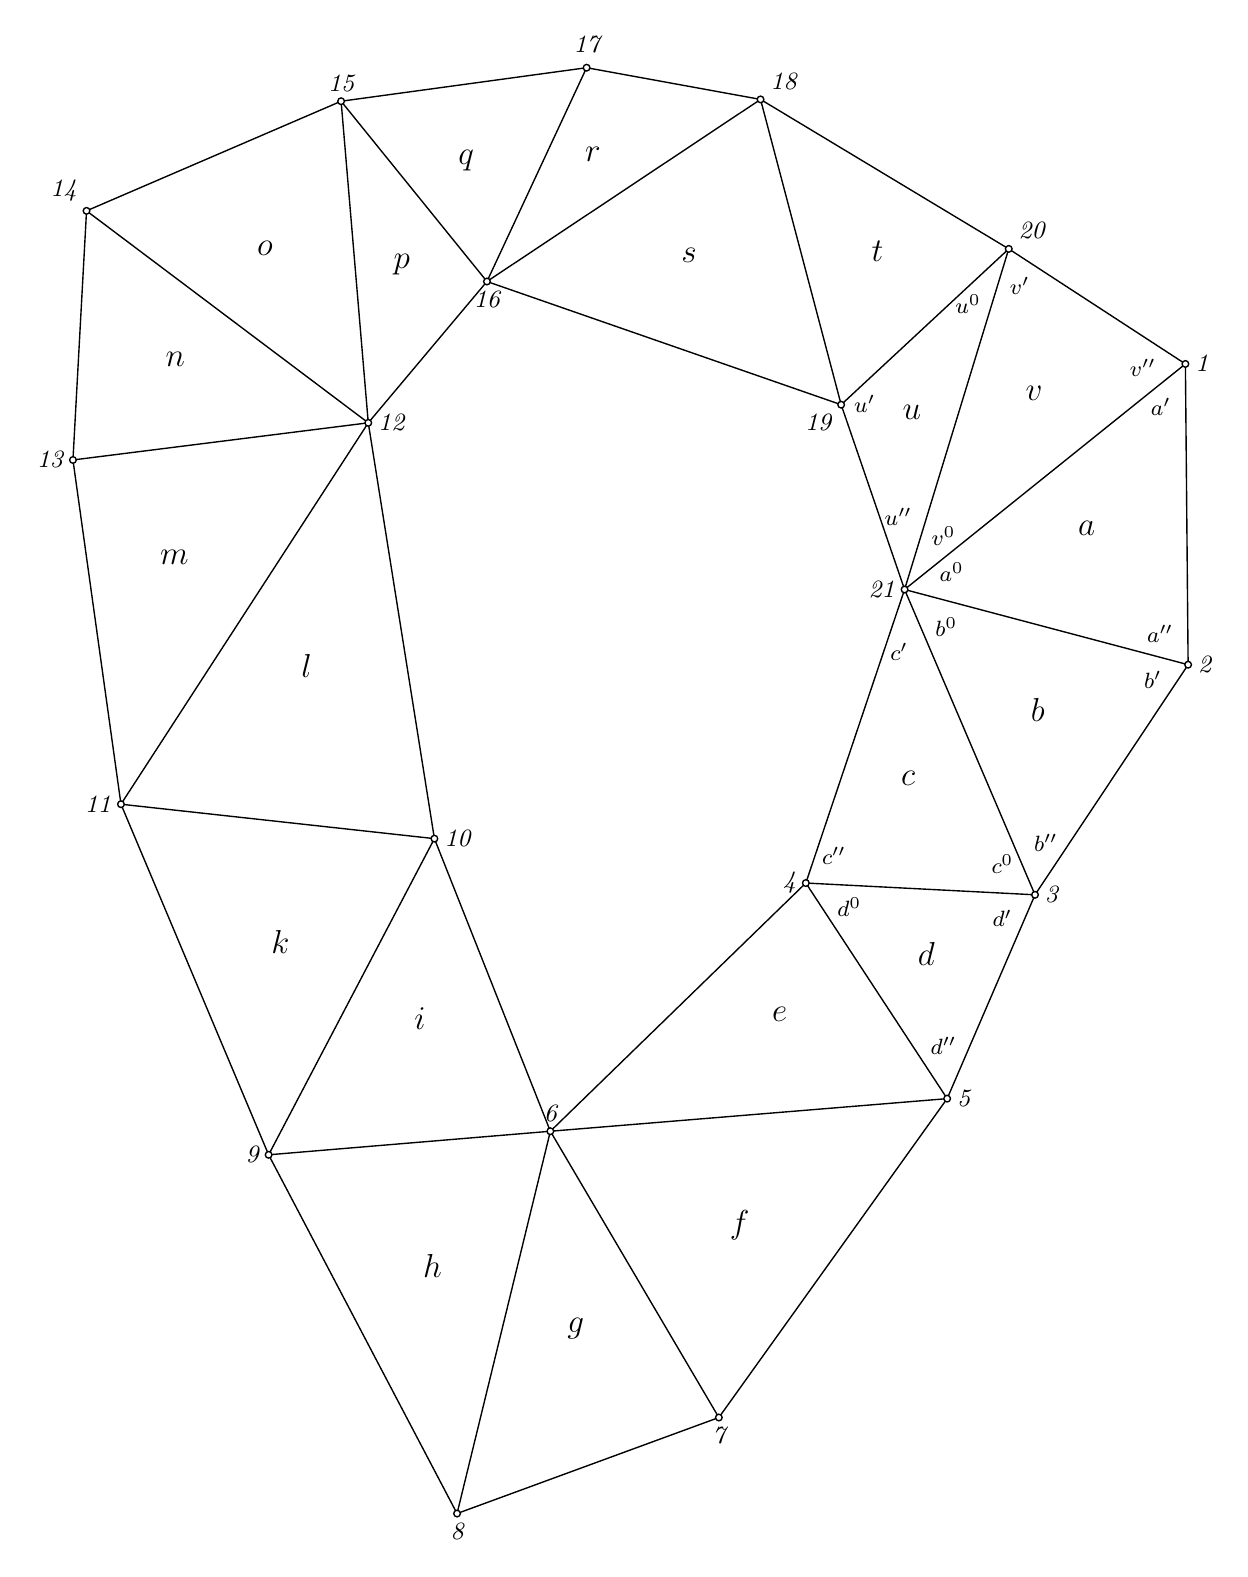
\begin{tikzpicture}[x=.0115cm,y=-.0115cm,line width=.5pt]
\coordinate (O1) at (1283,419);
\coordinate (O2) at (1286,751);
\coordinate (O3) at (1117,1005);
\coordinate (O4) at (864,992);
\coordinate (O5) at (1020,1230);
\coordinate (O6) at (582,1266);
\coordinate (O7) at (768,1582);
\coordinate (O8) at (479,1688);
\coordinate (O9) at (271,1292);
\coordinate (O10) at (454,943);
\coordinate (O11) at (108,905);
\coordinate (O12) at (381,484);
\coordinate (O13) at (55,525);
\coordinate (O14) at (70,250);
\coordinate (O15) at (351,129);
\coordinate (O16) at (512,328);
\coordinate (O17) at (622,92);
\coordinate (O18) at (814,127);
\coordinate (O19) at (903,464);
\coordinate (O20) at (1088,292);
\coordinate (O21) at (973,668);
\draw (O1)--(O2)--(O3)--(O5)--(O7)--(O8)--(O9)--(O11)--(O13)--(O14)--(O15)--(O17)--(O18)--(O20)--cycle;
\draw (O4)--(O6)--(O10)--(O12)--(O16)--(O19)--(O21)--cycle;
\draw (O21)--(O1) (O21)--(O2) (O21)--(O3) (O4)--(O3) (O4)--(O5);
\draw (O6)--(O5) (O6)--(O7) (O6)--(O8) (O6)--(O9);
\draw (O10)--(O9) (O10)--(O11) (O12)--(O11) (O12)--(O13) (O12)--(O14) (O12)--(O15);
\draw (O16)--(O15) (O16)--(O17) (O16)--(O18) (O19)--(O18) (O19)--(O20) (O21)--(O20);
\foreach \n in {1,...,21}{\draw[fill=white] (O\n) circle[radius=1.2pt];}
\node[right,font=\small\itshape] at (O1) {1};
\node[right,font=\small\itshape] at (O2) {2};
\node[right,font=\small\itshape] at (O3) {3};
\node[left,font=\small\itshape] at (O4) {4};
\node[right,font=\small\itshape] at (O5) {5};
\node[above,font=\small\itshape] at (O6) {6};
\node[below,font=\small\itshape] at (O7) {7};
\node[below,font=\small\itshape] at (O8) {8};
\node[left,font=\small\itshape] at (O9) {9};
\node[right,font=\small\itshape] at (O10) {10};
\node[left,font=\small\itshape] at (O11) {11};
\node[right,font=\small\itshape] at (O12) {12};
\node[left,font=\small\itshape] at (O13) {13};
\node[above left,font=\small\itshape] at (O14) {14};
\node[above,font=\small\itshape] at (O15) {15};
\node[below,font=\small\itshape] at (O16) {16};
\node[above,font=\small\itshape] at (O17) {17};
\node[above right,font=\small\itshape] at (O18) {18};
\node[below left,font=\small\itshape] at (O19) {19};
\node[above right,font=\small\itshape] at (O20) {20};
\node[left,font=\small\itshape] at (O21) {21};
\foreach \lab/\x/\y in {a/1174/601,b/1120/801,c/977/876,d/997/1070,e/835/1137,f/791/1370,g/610/1484,h/452/1415,i/438/1142,k/284/1057,l/313/752,m/167/632,n/168/414,o/267/291,p/418/309,q/489/194,r/629/188,s/735/299,t/943/295,u/981/472,v/1116/451}{\node[font=\large] at (\x,\y) {$\lab$};}
\node[font=\footnotesize] at (1025,649) {$a^{0}$};
\node[font=\footnotesize] at (1256,466) {$a'$};
\node[font=\footnotesize] at (1255,717) {$a''$};
\node[font=\footnotesize] at (1019,710) {$b^{0}$};
\node[font=\footnotesize] at (1247,768) {$b'$};
\node[font=\footnotesize] at (1129,948) {$b''$};
\node[font=\footnotesize] at (1081,971) {$c^{0}$};
\node[font=\footnotesize] at (967,737) {$c'$};
\node[font=\footnotesize] at (895,962) {$c''$};
\node[font=\footnotesize] at (912,1019) {$d^{0}$};
\node[font=\footnotesize] at (1081,1031) {$d'$};
\node[font=\footnotesize] at (1016,1172) {$d''$};
\node[font=\footnotesize] at (1043,353) {$u^{0}$};
\node[font=\footnotesize] at (929,463) {$u'$};
\node[font=\footnotesize] at (966,588) {$u''$};
\node[font=\footnotesize] at (1016,609) {$v^{0}$};
\node[font=\footnotesize] at (1100,333) {$v'$};
\node[font=\footnotesize] at (1236,423) {$v''$};
\end{tikzpicture}
\end{center}
